%for search with vim and okular
\synctex=1


%%=====================================================================================
% Settings
%%=====================================================================================
\newcommand{\mypapersize}{A4}
\newcommand{\mylaterality}{twoside} %% "oneside" or "twoside"
\newcommand{\myparskip}{half}
\newcommand{\myfontsize}{10pt}
\newcommand{\mylinespread}{singlespacing} % e.g.onehalfspacing, doublespacing, singlespacing
\newcommand{\mylanguage}{french} %american

\documentclass[%
  fontsize=\myfontsize,
	paper=\mypapersize,
	parskip=\myparskip,
	DIV=calc,
	headinclude=true,
	footinclude=true,
	open=right,
	appendixprefix=true,	% include appendix?
	bibliography=totoc,		% include an unnumbered unit of bibliography to the table of contents
	BCOR=10mm,        	  % binding correction (depends on how you bind
	\mylaterality,        % alternative: twoside
  \mylanguage
]{scrbook}

%Encoding
\usepackage[utf8]{inputenc}
\usepackage[T1]{fontenc}

\usepackage{float}

% language adaptions
\usepackage[\mylanguage]{babel}

%% general metadata:
\newcommand{\myauthor}{Manon Racine}  %% also used for PDF metadata (hyperref)
\newcommand{\mydocumentsubject}{Projet d'approfondissement}
\newcommand{\mysubject}{AI-enhanced LoRa Based Indoor Localization System}  %% also used for PDF metadata (hyperref)
\newcommand{\myshortsubject}{AI-enhanced LoRa Based Indoor Localization System}  %% also used for PDF metadata (hyperref)
%%\newcommand{\mykeywords}{Pedestrian detection, Deep learning, CNN, BonsEyes, Thermal images}  %% also used for PDF metadata (hyperref)

%% this information is used only for generating the title page:
\newcommand{\myuniversity}{HES-SO Master} %% your university/school
\newcommand{\myfaculty}{HE-Arc} %% your university/school

\newcommand{\mysupervisora}{Dr. Nuria Pazos}
%%\newcommand{\mysupervisorb}{Florian Sauser}

%%\newcommand{\myexpert}{Adrien Birbaumer}
%%=====================================================================================
% Colors
%%=====================================================================================
% includes some colors
\usepackage[table,usenames,dvipsnames]{xcolor}
\usepackage{color, colortbl}


% Define some colors used in the template
\definecolor{grey}{gray}{0.95}
\definecolor{dkgreen}{rgb}{0,0.6,0}

\definecolor{mauve}{rgb}{0.58,0,0.82}
\definecolor{red}{rgb}{1,0,0}
\definecolor{DispositionColor}{RGB}{0, 0, 0}


\definecolor{Red200}{HTML}{EF9A9A}
\definecolor{Red300}{HTML}{E57373}
\definecolor{Red500}{HTML}{ F44336}
\definecolor{Red800}{HTML}{ C62828}

\definecolor{Orange800}{HTML}{ EF6C00}

\definecolor{Teal900}{HTML}{004D40}
\definecolor{Teal800}{HTML}{00695C}
\definecolor{Teal200}{HTML}{80CBC4}


\definecolor{Cyan200}{HTML}{80DEEA}
\definecolor{Cyan800}{HTML}{ 00838F}

\definecolor{Blue900}{HTML}{0D47A1}
\definecolor{Blue800}{HTML}{1565C0}
\definecolor{Blue700}{HTML}{1976D2}
\definecolor{Blue600}{HTML}{1E88E5}
\definecolor{Blue500}{HTML}{2196F3}
\definecolor{Blue400}{HTML}{42A5F5}
\definecolor{Blue300}{HTML}{64B5F6}
\definecolor{Blue200}{HTML}{90CAF9}
\definecolor{Blue100}{HTML}{BBDEFB}

\definecolor{Green900}{HTML}{1B5E20}
\definecolor{Green800}{HTML}{2E7D32}

\definecolor{Grey100}{HTML}{F5F5F5}



%%=====================================================================================
%% includes pictures --> possible to include them in header/footer
%%=====================================================================================
\usepackage[pdftex]{graphicx}


%%=====================================================================================
%% Style
%%=====================================================================================
% override some list packages that they use babel -> see koma script doc
\usepackage{scrhack}

% nicer quotes
\usepackage[%
  autostyle,          % adapts language setting
  strict,             % turns warnings into errors
  english=american    % use american quotes style
]{csquotes}

\usepackage[automark]{scrpage2}							% allows usage of header and footer
\usepackage[perpage, hang]{footmisc} 				% footnote options

\renewcommand{\headfont}{\normalfont\sffamily\color{DispositionColor}}
\renewcommand{\pnumfont}{\normalfont\sffamily\color{DispositionColor}}
\addtokomafont{disposition}{\color{DispositionColor}}
\addtokomafont{caption}{\color{DispositionColor}\footnotesize}
\addtokomafont{captionlabel}{\color{DispositionColor}}

\usepackage{calc} %% used for calculation of header footer etc. ...

%% change page layout
\addtolength{\oddsidemargin}{-.875in}
\addtolength{\evensidemargin}{-.875in}
\addtolength{\textwidth}{1.75in}
\addtolength{\topmargin}{-.875in}
\addtolength{\textheight}{3in}  %1.75

% header and footer
\pagestyle{scrheadings}							% for customization for header and footer
\renewcommand{\chapterpagestyle}{scrheadings}	% include header and footer on chapter pages
\clearscrheadfoot

% http://ctan.uib.no/macros/latex/contrib/koma-script/doc/scrguien.pdf
% page 204
\ihead{\myshortsubject}
\ohead{Public}
\ifoot{\vspace{-0.25cm}\myauthor}
\ofoot{ \vspace{-0.25cm} \thepage}
\automark{chapter}
\setheadsepline[ \textwidth + 5pt ]{1pt} % seperation line for header...
\setfootsepline[ \textwidth + 5pt ]{1pt} % ... and footer
\setkomafont{footsepline}{\color{red}} 	 % change colors of seperation lines
\setkomafont{headsepline}{\color{red}}

%%=====================================================================================
%% Table on Contents
%%=====================================================================================
\setcounter{tocdepth}{2}
\setcounter{secnumdepth}{2} % change la profondeur de numérotation

\usepackage{makecell}

\usepackage{tabulary}
\newcolumntype{K}[1]{>{\centering\arraybackslash}p{#1}}

\usepackage{verbatim}


%%=====================================================================================
%% bibliography with biber/biblatex
%%=====================================================================================
\usepackage[backend=bibtex, %% using "biber" to compile references (instead of "biblatex")
            style=numeric, %% see biblatex documentation
            style=alphabetic, %% see biblatex documentation
            backref=true, %% create backlings from references to citations
            natbib=true, %% offering natbib-compatible commands
            hyperref=true,
            sorting=none, %% using hyperref-package references
]{biblatex}

%\addbibresource{../bib/bibliography.bib}
\addbibresource{bib/bibliography.bib}
%\addbibresource{bib/bibliography_VAL.bib}

%%=====================================================================================
%% SIUNITSX -- simplified usage of SI-units
%%=====================================================================================
%\usepackage[
%            group-digits=false,
%            exponent-product = \cdot, % use \cdot instead * for exponent product
%            binary-units=true,
%            load-configurations=binary,
%            load-configurations=abbreviations,
%]{siunitx}

% Easy typesetting hex and bin and oct
\usepackage[autolanguage, nosepfour]{numprint}
\usepackage{nbaseprt}

%%=====================================================================================
%% ifthen and todonotes puts to-do-notes in the printed document if you want
%%=====================================================================================
%% used to disable todonotes package
\usepackage{ifthen}
\newboolean{myaddlistoftodos}
\newboolean{showconfidential}

\reversemarginpar %To display the todo in the right margin
\setlength{\marginparwidth}{2cm} %To correct the bad placement

\usepackage[english]{todonotes}

%%=====================================================================================
%% Tables, figures, enums, etc...
%%=====================================================================================
%% nice rule's for tables try \toprule \midrule \bottomrule
\usepackage{booktabs}

%% set width of table and more
\usepackage{tabularx}										% creates tables

%% rotate tables and figures
\usepackage{rotating}

%% define caption style
\addtokomafont{caption}{\small} 	% small captions
\usepackage[font=small, width=0.9\textwidth, format=plain, labelfont=bf]{caption}

%%
\usepackage{subfigure}
\usepackage{placeins}

%% customize item look
\usepackage{enumitem}

%%=====================================================================================
%% some utility stuff
%%=====================================================================================
% improved typographical settings
\usepackage[%
    protrusion=true, %
    factor=900       %
]{microtype}

%% switch of extra space after punctuation
\frenchspacing

%% switches to Palatino with small caps and old style figures
\usepackage[%
            sc,%
            osf,%
]{mathpazo}

%% kills space between items
\setlist{noitemsep}

%doc% For additional special characters available by \verb#\ding{}#
\usepackage{pifont}  %% Sonderzeichen fuer Titelseite \ding{}

%doc% This package is required for intelligent spacing after commands
\usepackage{xspace}

%doc% This package offers strikethrough command \verb+\sout{foobar}+.
\usepackage[normalem]{ulem}

%% prevent club & widow penalty
\clubpenalty10000
\widowpenalty10000
\displaywidowpenalty10000

%% Titlepage
\usepackage{tcolorbox}


%%=====================================================================================
%% lslistening: used to include source code
%%=====================================================================================
\usepackage{listings}				% include source code

\lstset{% 							% options for representation of source code
  backgroundcolor=\color{grey},   % choose the background color; you must add \usepackage{color} or \usepackage{xcolor}
  basicstyle=\footnotesize,        % the size of the fonts that are used for the code
  breakatwhitespace=false,         % sets if automatic breaks should only happen at whitespace
  breaklines=true,                 % sets automatic line breaking
  captionpos=b,                    % ses the caption-position to bottom
  commentstyle=\color{dkgreen}, % comment style
  deletekeywords={...},            % if you want to delete keywords from the given language
  escapeinside={\%*}{*)},          % if you want to add LaTeX within your code
  frame=lines,                     % adds a frame around the code
  keepspaces=true,                 % keeps spaces in text, useful for keeping indentation of code (possibly needs columns=flexible)
  keywordstyle=\color{blue},       % keyword style
  language=C,                      % the language of the code
  morekeywords={*,...},            % if you want to add more keywords to the set
  numbers=left,                    % where to put the line-numbers; possible values are (none, left, right)
  numbersep=8pt,                   % how far the line-numbers are from the code
  numberstyle=\tiny\color{gray},   % the style that is used for the line-numbers
  rulecolor=\color{black},         % if not set, the frame-color may be changed on line-breaks within not-black text (e.g. comments (green here))
  showspaces=false,                % show spaces everywhere adding particular underscores; it overrides 'showstringspaces'
  showstringspaces=false,          % underline spaces within strings only
  showtabs=false,                  % show tabs within strings adding particular underscores
  stepnumber=1,                    % the step between two line-numbers. If it's 1, each line will be numbered
  stringstyle=\color{blue},        % string literal style
  tabsize=2,                       % sets default tabsize to 2 spaces
  title=\lstname,                  % show the filename of files included with \lstinputlisting; also try caption instead of title
}

%theme for C
\lstdefinestyle{C}{
	language=c, showspaces=false,
	keywordstyle=		\color{blue}\scriptsize,
	commentstyle=	  \color{dkgreen}\scriptsize\sffamily,
	stringstyle=		\color{mauve}\scriptsize,
	title=\lstname,
	escapeinside={//(*}{*)},
	morekeywords={},
	numbers = left, numberstyle=\tiny\color{black}
}

\usepackage{setspace} 
\usepackage{blindtext}
\usepackage{graphicx}
\usepackage[export]{adjustbox}

\usepackage[top=2.5cm, bottom=3cm, left=2.5cm, right=2cm]{geometry}

%%=====================================================================================
%% pdfcompresslevel from 0 to 10; std is fine
%%=====================================================================================
\pdfcompresslevel=9

%%=====================================================================================
%% Hyperref should always be the last package added --
%%=====================================================================================
\usepackage{hyperref}								% should be the last package to be inlcuded!

%\usepackage[%							% enables typesettings for hyperlinks
%pdftitle={\mysubject},%
%pdfauthor = {\myauthor},%
%pdfsubject = {\mysubject},%
%colorlinks={false},
%pdfcreator={pdfTex},%
%pdfkeywords={\mykeywords},%
%pdftex = true,%
%backref,%
%pagebackref=false, % creates backward references too
%bookmarks=True, %
%bookmarksopen=false, % when starting with AcrobatReader, the Bookmarkcolumn is opened
%pdfpagemode=UseOutlines,% None, UseOutlines, UseThumbs, FullScreen
%plainpages=false % correct, if pdflatex complains: ``destination with same identifier already exists''
%]{hyperref}								% should be the last package to be inlcuded!

%---------------------------------------------------------------------------------------------------
% include figures
%---------------------------------------------------------------------------------------------------
\newcommand{\myfigsrc}[5]{
\begin{figure}[htp]
	\begin{center}
		\includegraphics[width=#2\textwidth]{figures/#1}
		\captionsource{#3}{#4}
		\label{#5} %% NOTE: always label *after* caption!
	\end{center}
\end{figure}
}

\newcommand{\myfig}[4]{
\begin{figure}[htp]
	\begin{center}
		\includegraphics[width=#2\textwidth]{figures/#1}
		\caption[#3]{#3}
		\label{#4} %% NOTE: always label *after* caption!
	\end{center}
\end{figure}
}

\newcommand{\mypdfsrc}[6]{
\begin{figure}[htp]
	\begin{center}
		\includegraphics[page=#6, width=#2\textwidth, frame]{figures/#1}
		\captionsource{#3}{#4}
		\label{#5} %% NOTE: always label *after* caption!
	\end{center}
\end{figure}
}


\newcommand*{\captionsource}[2]{%
\caption[{#1}]{%
	#1%
	\\\hspace{\linewidth}%
	\textbf{Source:} #2%
}%
}



%% ========================================================================
%%  TODO: Enable/Disable
%% ========================================================================
\setboolean{myaddlistoftodos}{false}  %% "true" or "false"
%% If set to "true": the current list of open todos is added after the
%% table of contents. If \mytodonotesoptions is set to "disable", no
%% list of todos is added, independent of this setting here.


%----------------------------------------------------------------------------------------
%	\begin{document}
%----------------------------------------------------------------------------------------
\begin{document}

\frontmatter

\begin{titlepage}
	
	% MSE + HES-SO Images
	\vspace{-1cm}
	\begin{minipage}{0.49\textwidth}
		\begin{flushleft} \large
			
\includegraphics[width=0.8\textwidth]{figures/titlepage_fig/mse.pdf}
		\end{flushleft}
	\end{minipage}
	\begin{minipage}{0.5\textwidth}
		\begin{flushright} \large
			
\includegraphics[width=0.6\textwidth]{figures/titlepage_fig/hesso2.pdf}
		\end{flushright}
	\end{minipage}
	
	% HES-SO Master postal address
	\begin{flushleft}
		\footnotesize 		
		Master of Science HES-SO in Engineering\\
		Av. de Provence 6\\CH-1007 Lausanne
	\end{flushleft}
	
	% Vertical space under HES-SO Master postal address
	\vspace{1.7cm}
	
	\begin{flushright}
		{\huge Master of Science HES-SO in Engineering}
		
		\vspace{0.5cm}
		{\Large Orientation : Technologies de l’information et de la communication (TIC)}
		
		\vspace{1.7cm}

		\begin{spacing}{2.0}
			{\Huge \mysubject}
		\end{spacing}

		\vspace{1cm}
		\begin{spacing}{2.0}	
			Fait par\\
			{\huge \myauthor}
		\end{spacing}
	
		
		\vspace{1cm}
		\begin{spacing}{1.5}
			Sous la direction de\\
			{\Large \mysupervisora }\\ 
			%{\Large \mysupervisorb }
		\end{spacing}
	
		{\Large \myfaculty}

%		\begin{spacing}{1.5}
%			Expert externe\\
%			{\Large \myexpert }
%		\end{spacing}
		
		\vspace{1cm}%% Date
		{\large St-Imier, HE-Arc, \today}
	\end{flushright}
	% Bottom of the page
\end{titlepage}
\cleardoublepage
%\chapter*{Soumission du projet}
Accepté par la HES-SO//Master (Suisse, Lausanne) sur proposition de

\vspace{0.5cm}
Dr. Nuria Paszos conseillère de travail de Master

\vspace{2cm}
St-Imier, le 18.09.2018

\vspace{1.5cm}
\begin{minipage}[t]{0.5\textwidth}
	\raggedright
	Dr. Nuria Pazos\\
	Conseillère
\end{minipage}%
\begin{minipage}[t]{0.45\textwidth}
%	\raggedleft
	Prof. Didier Rizzotti\\
	Responsable de la filière MRU-TIC
\end{minipage}




\cleardoublepage

%----------------------------------------------------------------------------------------
%	Abstract
%----------------------------------------------------------------------------------------
%\chapter{Résumé}
Ce document présente une analyse de sécurité axée sur le bus CAN d'un véhicule autonome conçu par la société Navya.

Les premiers chapitres décrivent une analyse de l'état de l'art des moyens de communication utilisés dans les véhicules, qu'ils soient autonomes ou à conduite manuelle, puis se focalisent ensuite sur les communications employant le bus CAN, en expliquant les problèmes de sécurité qui peuvent être rencontrés en se basant sur les concepts généraux du chiffrement des télécommunications. 

Cette analyse explore ensuite l'architecture d'un véhicule autonome et la problématique en cas d'accès physique au bus CAN qui n'est pas protégé nativement contre les intrusions et attaques diverses.

Ensuite, des mesures physiques sur le bus CAN contrôlant la direction du véhicule démontrent effectivement la transmission en clair des informations, sans vérification de l'intégrité.

Pour terminer, différentes solutions applicables sont présentées, ainsi qu'une proposition de surcouche pour un bus CAN permettant de garantir l'intégrité et l'authentification des données transférées.
disposition de la documentation nécessaire.

{\let\clearpage\relax\par \chapter{Abstract}}
Dafuq is that report ?
%\chapter{Remerciements}
Merci Jackie
%\chapter*{Déclaration}

\noindent Je, soussigné, \myauthor, déclare sur l’honneur que le travail rendu, intitulé \enquote{\mysubject} est le fruit d’un travail personnel. Je certifie ne pas avoir eu recours au plagiat ou à toutes autres formes de fraudes. Toutes les sources d’information utilisées et les citations d’auteur ont été clairement mentionnées.


\vspace{2cm}

%% definition of the block tat contains date and signature
\newcommand{\mysignatureblock}[3]{%
	%% Sorry, this is a "bit" of a hack. Maybe someone knows a more elegant method?
	\begin{tabular}{llp{2em}l} 
		#1 & \hspace{4cm}        & & \hspace{4cm} \\\cline{2-2}\cline{4-4}
		&                     & & \\[-3mm]
		& {\footnotesize #2}  & & {\footnotesize #3}
	\end{tabular}
}

\mysignatureblock{St-Imier,}{Date}{Signature}



%----------------------------------------------------------------------------------------
%	List of Contents/Figures/Tables
%----------------------------------------------------------------------------------------
\tableofcontents
\listoffigures

\ifthenelse{\boolean{myaddlistoftodos}}{
  \newpage\todototoc \listoftodos          %% handy if you are using todonotes with \todo{}
}{}

%----------------------------------------------------------------------------------------
%	Body
%----------------------------------------------------------------------------------------
\mainmatter

% Chapter file here
%
\chapter{Rapport intérmédiaire : 17.09.2018 au 12.10.2018}

Ce premier résumé a pour but de poser le projet et d'étudier l'état de l'art. Depuis les lectures concernant ce qu'il existe en machin learning pour le positionnement indoor, il est nécessaire de faire un résumé afin de choisir le meilleur algorithme afin d'améliorer le positionnement indoor à l'aide de la technologie LoRa et le mode ranging.

\section{Cahier des charges}
\subsection{Introduction}
Les systèmes de localisation basés sur GPS souffrent de la détérioration de la précision et sont presque indisponibles dans les environnements intérieurs. Pour les environnements intérieurs, de nombreuses technologies de systèmes de positionnement ont été conçues sur la base de la vision, de la détection infrarouge ou ultrasonore, des champs magnétiques de la terre, des accéléromètres / gyromètres, des balises BLE ou de la communication WiFi. Chacune de ces technologies existantes a des coûts, une précision et un compromis maximum en matière de couverture, mais un service de localisation intérieur générique reste difficile à obtenir.

\subsection{But du projet}
S'appuyant sur les capacités étendues des nouveaux circuits intégrés LoRa, ce projet développera et déploiera un système de localisation capable d'améliorer la précision de la position atteinte par les systèmes de localisation basés sur LoRa existants reposant sur des mécanismes TDOA ou de télémétrie. À cette fin, une exploration et une comparaison des différentes techniques "machine learning/deep learning" pour le positionnement basé sur le "fingerprinting" seront effectuées.


\subsection{Objectifs et tâches à réaliser}
\begin{enumerate}
	\item Etudier le cahier des charges
	\item Etudier l’état de l’art des techniques à utiliser dans le cadre du projet, en particulier les systèmes de localisation indoor basés sur des techniques d’apprentissage, et réunir une documentation (env. 20% effort)
	\item Etablir un planning pour l’ensemble du projet.
	\item Définir un plan des tests à effectuer.
	\item Définir les procédures de test
	\item Définir le setup pour la collecte de données de localisation
	\item Prise en main de l’environnement de développement pour les phases de training et du test de la technique d’apprentissage retenue (e.g., PyTorch).
	\item Implémentation de la solution ML retenue.
	\item Tester le système selon le protocole préétabli.
	\item Faire des propositions pour améliorer les performances de l’algorithme et, si possible, les implémenter.
	\item Rédiger le rapport et documenter l’ensemble du projet.
\end{enumerate}


\section{Résumé du document 00}
Ce document décrit la localisation sans utiliser le GPS et en utilisant LoRa. Il a surtout été utile d'utiliser ce document pour la gestion des "outliers"
\\
\\
Le problème principal avec le GPS c'est la consommation et la durée de vie c'est pourquoi un système basé sur LoRa a été étudié. La portée en milieu rural est d'environ 15km alors qu'il est de 5km dans un milieu urbain cela grâce à la bonne sensibilité du récepteur (-130dBm). Une chose intéressant est la bande passante qui est plus large que d'autres technologies qui permet de distinguer différents chemins du même signal. Sagemcom ont obtenus des bons résultats au niveau de la précision qui est de environ 4 mètres. 
\\
\\
Ce qui est intéressant c'est dans cette publication c'est la manière de traiter les "outliers - valeurs aberrante, c'est-à-dire les points qui ne sont pas cohérent lors d'une mesure. Selon Barnet et Lewis [11], un "outliers" est définit comme étant une observation qui semble incompatible avec le reste d'un ensemble de données.
Garder un "outliers" dans une set de données peut amener à de mauvais résultat il est donc important de les détecter correctement. Il existe différentes méthodes pour déterminer ces "outliers" :

\begin{enumerate}
	\item Grubbs' test : Détecte un "outliers" en supposant une distribution normale.
	\item Tietjen-Moore test : C'est une généralisation de Grubbs' test pour détecter de multiple outliers. Il a cependant un inconvénient, il est nécessaire de connaitre le nombre exact d'ouliers.
	\item Generalized Extreme Studentized Deviate (ESD): C'est également une généralisation du test Grubbs' mais il n'est pas nécessaire de connaitre à l'avance le nombre d'ouliers. Ce test nécessite uniquement une limite supérieure pour le nombre suspect d'outliers.[01]
\end{enumerate}

[11] V. Barnett; T. Lewis, Outliers in Statistical Data, 3rd ed. Wiley Series in Probability and Mathematical Statistics, 1994.

[01] lien concernant les ESD : https://www.itl.nist.gov/div898/handbook/eda/section3/eda35h3.htm

\section{Résumé du document 01}
Cette publication parle d'une analyse comparative entre différents algorithmes de "machine learning" pour du positionnement indoor. L'étude est basée sur un positionnement "fingerprint" ce qui permet de cartographier un endroit à l'aide du de la force du signal récéptionné (RSS - Received Signal Strength).
Dans cet article, les algorithmes de "machine learning" sélectionnés sont comparés en termes de précision de positionnement et de temps de calcul. la base de donnée UJIIndoorLoc a été utilisé pour les différentes expérimentation. Les résultats expérimentaux révèlent que l’algorithme k-Nearest Neighbor (k-NN) est le plus approprié lors du positionnement.

\subsection{Introduction}
Au cours des expériences, la base de données UJIIndoorLoc, qui est préparée pour les systèmes de positionnement à l'intérieur [8], est utilisée. La classification est effectuée en premier lieu en utilisant le jeu de données d'origine en considérant les valeurs RSS de 520 points d'accès sans fil (WAP) et les nouveaux attributs définis en tant que «cellule» qui composent les attributs BuildingID, Floor, SpaceID et RelativePos. Ensuite, une nouvelle méthode est proposée: «Séparation déductive pour le positionnement intérieur (DESIP - Deductive Separation for Indoor Positioning)». Dans cette méthode, tout d'abord, seules les informations de bâtiment et les valeurs RSS mesurées à partir de 520 WAP sont utilisées pour la tâche de classification.
\\
\\
Durant les expériences, des algorithmes déterministes tels que le plus proche voisin (NN - nearest neighbor), le SMO, l'arbre de décision (J48) et des algorithmes probabilistes tels que Naïve Bayes et Bayes Net sont utilisés. L’algorithme le plus approprié pour la solution du problème de positionnement intérieur est déterminé en comparant la précision et le temps de calcul de chaque approche.
\\
\\
La base de données entière est séparée de telle sorte que 19.937 enregistrements soient réservés à la formation et 1.111 enregistrements soient réservés aux tests. Il y a 529 caractéristiques et ces caractéristiques sont les coordonnées où sont prises les empreintes digitales WiFi, telles que bâtiment, étage, espace (bureau, laboratoire, etc.), position relative (dans une pièce ou dans un couloir), etc. Le jeu de données de formation UJIIndoorLoc comprenant les valeurs RSS de 520 WAP et un nouvel attribut «cellule» qui compose les attributs floor, buildingID, spaceID et relative position de l'ensemble de données d'origine est utilisé pour la tâche de classification. Les étapes des expériences utilisant ce jeu de données sont illustrées à la figure \ref{fig:newAttribute}.

\begin{figure}[H]
	\begin{center}
		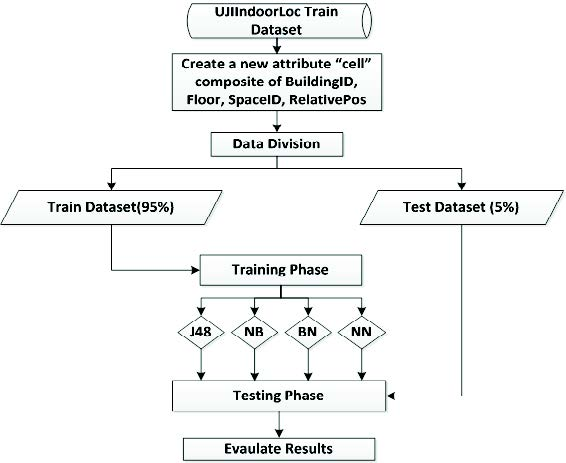
\includegraphics[scale=1]{figures/newattribute.jpg}
		\caption{The new attribute “cell” construction phase}
		\label{fig:newAttribute} %% NOTE: always label *after* caption!
	\end{center}
\end{figure}


\subsection{Algorithmes}
Dans la section suivante, les algorithmes de classification utilisés dans cette étude sont brièvement décrits.

\subsubsection{Decision Tree}
L'arbre de décisions et une méthode très connue en "machine learning". Il possède des noeuds de décisions (non-terminal), des branches, et des noeuds feuilles (terminal) qui représentent les caractéristiques, condition et les classes. A chaque noeud de décision on sait quelle branches suivre et lorsque l'algorithme atteint un noeud final, le label contenu dans ce même noeud est retourné comme étant la classe. 
L’ID3 de Quinlan et son successeur, C4.5, sont les plus populaires parmi les algorithmes d’arbre de décision [19].

(19) J. R. Quinlan, “ C4. 5: programs for machine learning”, Elsevier, 2014.

\subsubsection{Naïve Bayes}
Le classificateur Naïve Bayes [22] basé sur le théorème de Bayes est un algorithme d'apprentissage supervisé [23]. Il est robuste aux données bruyantes, facile à construire, affiche une grande précision et rapidité lorsqu'il est appliqué à de grandes bases de données et exécute des modèles de classification plus complexes. Par conséquent, il est largement utilisé dans les tâches de classification. Il calcule la probabilité de chaque attribut dans les données en supposant qu'elles sont également importantes et indépendantes les unes des autres. Cette hypothèse est appelée indépendance conditionnelle de classe [24, 25].
\\
\\
(22) G. H. John, and P. Langley, “Estimating Continuous Distributions in Bayesian Classifiers”, 11th Conference on Uncertainty in Artificial Intelligence, pp., 338-345, 1995.

(23) C. Anuradha, and S. Dhall, "Software Defect Prediction Using Supervised Learning Algorithm and Unsupervised Learning Algorithm", 2013.

(24) W. Yotsawat, and A. Srivihok, "Inbound tourists segmentation with combined algorithms using K-Means and Decision Tree”, 10th International Joint Conference on Computer Science and Software Engineering (JCSSE), pp.189-194, 2013.

(25) S. Ureerat, and P. Singsri, "The classifier model for prediction quail gender after birth based on external factors of quail egg", IEEE 11th International Joint Conference on Computer Science and Software Engineering (JCSSE), 2014.

\subsubsection{Bayesian Network}

L'algorithme de réseau bayésien est largement utilisé pour la classification et est basé sur le théorème de Bayes où la probabilité conditionnelle sur chaque nœud est calculée et forme un réseau bayésien. Il s'appelle également réseau de croyance ou réseau occasionnel. Réseau bayésien a deux parties nommées qualitatives et quantitatives, qui sont la structure topologique du réseau bayésien et le tableau de probabilité conditionnelle (CPT), respectivement [26].

Le réseau bayésien est un graphe acyclique dirigé où chaque nœud représente un attribut des données et un ensemble de distributions de probabilité. Ces distributions donnent les probabilités pour la valeur de chaque nœud étant donné que les parents de nœud.

(26) D. Yang, and L. Jin-lin, "Research on personal credit evaluation model based on bayesian network and association rules", 2007 International Conference on Wireless Communications, Networking and Mobile Computing, 2007.

\subsubsection{K-Nearest Neighbor}
Le classificateur K-Nearest Neighbor (K-NN) [27] est également connu sous le nom de classificateur basé sur la distance qui classe les instances en fonction de leur similarité. C'est l'un des algorithmes les plus populaires de l'apprentissage automatique. C'est un type d'apprentissage paresseux dans lequel la fonction n'est approchée que localement et tout calcul est retardé jusqu'à la classification. Le tuple inconnu dans K-NN est assigné à la classe la plus commune parmi ses K-plus proches voisins. Lorsque K = 1, le tuple inconnu se voit attribuer la classe du tuple d'apprentissage le plus proche dans l'espace des motifs [28].

(27) D. W. Aha, D. Kibler , and M. K. Albert, “ Instance-based learning algorithms”, Machine Learning, vol. 6, pp., 37-66, 1991.

(28) C. Shah, and A. G. Jivani, "Comparison of data mining classification algorithms for breast cancer prediction", 2013 Fourth International Conference on Computing, Communications and Networking Technologies (ICCCNT), pp.1-4, 2013.

\subsubsection{SMO}
L'algorithme d'optimisation séquentielle minimale (SMO - Sequential minimal optimization) [29] est représenté par John C. Platt pour la formation du classificateur de vecteurs de support à l'aide des noyaux polynomiaux ou RBF. C'est l'un des algorithmes les plus courants pour la classification des grandes marges par SVM. Il remplace globalement toutes les valeurs manquantes et transforme les attributs nominaux en attributs binaires. La SVM est une technique de classification basée sur la technologie des réseaux neuronaux utilisant la théorie de l'apprentissage statistique [30]. Il recherche un hyperplan optimal linéaire afin de maximiser la marge de séparation entre la classe positive et la classe négative. En pratique, la plupart des données ne sont pas linéairement séparables; ainsi, pour rendre la séparation possible, la transformation est effectuée à l'aide d'une fonction du noyau. L'entrée est transformée en un espace caractéristique de dimension supérieure à l'aide d'une cartographie non linéaire [30]. Une décision sur la fonction du Kernel est nécessaire pour implémenter SVM. Le Kernel définit la classe de fonction [31].

[29] J. Platt, “Fast Training of Support Vector Machines using Sequential Minimal Optimization”, Advances in Kernel Methods - Support Vector Learning, 1998.

[30] P. Niken, and H. Ohwada, "Applicability of machine-learning techniques in predicting customer defection", IEEE 2014 International Symposium on Technology Management and Emerging Technologies (ISTMET), 2014.

[31] S. M. Obaidullah, K. Roy, and N. Das, "Comparison of different classifiers for script identification from handwritten document", 2013 IEEE International Conference on Signal Processing, Computing and Control (ISPCC), pp.1-6, 2013.

\subsubsection{AdaBoost}
AdaBoost (Adaptive Boosting) [32] est un algorithme d'apprentissage d'ensemble. Généralement, il peut être utilisé avec des algorithmes de Machine learning faibles pour améliorer leurs performances. Il est simple à mettre en œuvre, rapide et moins susceptible d'avoir un overfitting. Il améliore les algorithmes de classification instables tels que J48, DecisionStump, etc. L'idée derrière cet algorithme est d'obtenir un classificateur très précis en combinant de nombreux classificateurs faibles. Il fonctionne en exécutant de manière répétée un algorithme d'apprentissage faible donné sur diverses distributions sur les données d'apprentissage, puis en combinant les classificateurs produits par l'apprenant faible en un classificateur composite unique [33]. Les classificateurs de l'ensemble sont ajoutés un par un, de sorte que chaque classificateur suivant est entrainé sur des données difficiles pour les membres précédents de l'ensemble. Les poids sont définis sur les instances du jeu de données, en suivant une règle selon laquelle les instances difficiles à classer prennent plus de poids. Cette règle conduit les classificateurs ultérieurs à se concentrer sur eux [34].

[32] Y. Freund, and R. E. Schapire, “Experiments with a new boosting algorithm”, 3th International Conference on Machine Learning, San Francisco, pp. 148-156, 1996.

[33] R. Shams, and R. E. Mercer, "Classifying Spam Emails Using Text and Readability Features", 2013 IEEE 13th International Conference on Data Mining (ICDM, pp. 657-666, 2013.

[34] S. O. Sharif, L. I. Kuncheva, and S. P. Mansoor, "Classifying encryption algorithms using pattern recognition techniques", 2010 IEEE International Conference on Information Theory and Information Security (ICITIS), , pp. 1168-1172, 2010.

\subsubsection{Bagging}
le Bagging [35] crée des sacs de données de la même taille que le jeu de données d'origine en appliquant une sélection aléatoire à différents sous-ensembles des données d'apprentissage avec de nombreux exemples qui apparaissent plusieurs fois. Ce processus est appelé réplication bootstrap des données d'entrainement. L'idée derrière cette technique est de construire différents classificateurs en utilisant ces sous-ensembles. Chaque sous-ensemble est utilisé pour entrainer un classificateur individuel. Cette approche d'ensemble utilise le nombre de classificateurs a priori [35].

[35] L. Breiman, “Bagging predictors”, Machine Learning. vol. 24, no. 2, pp.123-140, 1996.

\subsection{Conclusions}
Dans cet article les algorithme suivant ont été comparé : NN, SMO, J48, Naïve Bayes and BayesNet.

Lorsque tout le dataset est pris en compte, c'est l'algorithme J48 qui est le meilleur :

\begin{figure}[H]
	\begin{center}
		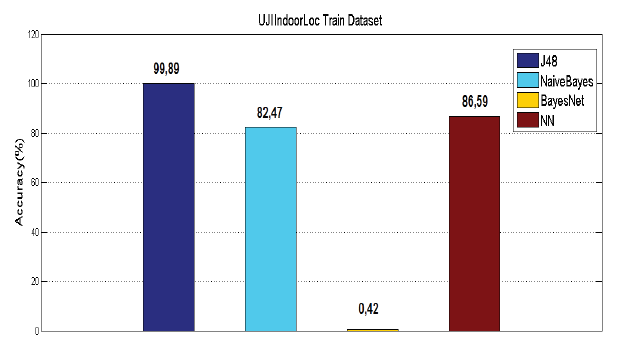
\includegraphics[scale=1]{figures/wholeDataset.png}
		\caption{Accuracy results of classification using whole dataset}
		\label{fig:wohledataset} %% NOTE: always label *after* caption!
	\end{center}
\end{figure}

Ensuite, en accordance à l'approche DESIP (Deductive Separation for Indoor Positioning), la classification est effectuée en 3 phases (building,floor and region). Le resultat des algorithme pour cette classification donne BayesNet comme étant le meilleur.

\begin{figure}[H]
	\begin{center}
		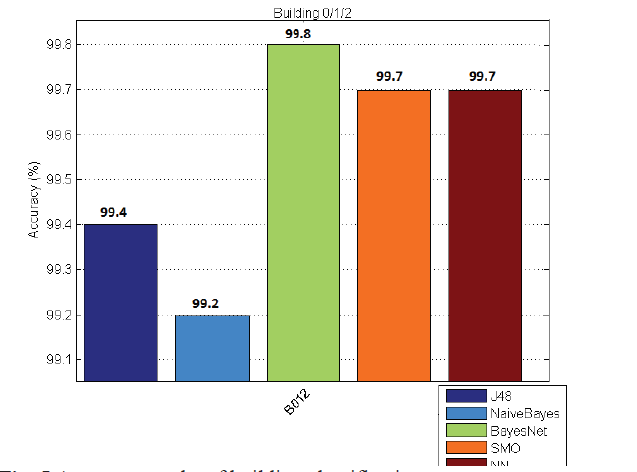
\includegraphics[scale=1]{figures/bluildingClassification.png}
		\caption{Accuracy results of building classification}
		\label{fig:builClass} %% NOTE: always label *after* caption!
	\end{center}
\end{figure}

Suite à cela la classification a été faite en fonction des étages (floors). Dans ce cas le meilleur algorithme est NN. 

\begin{figure}[H]
	\begin{center}
		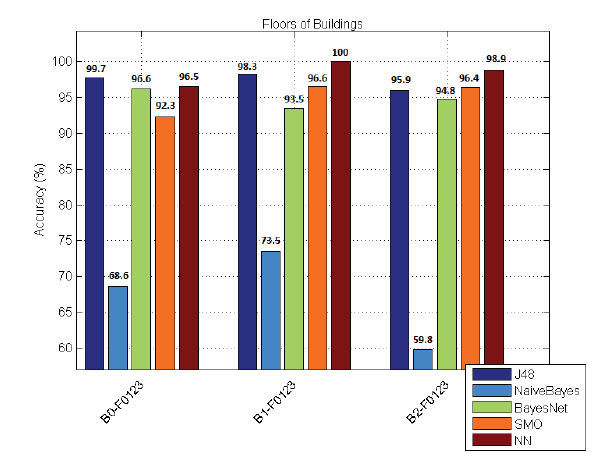
\includegraphics[scale=1]{figures/floorClassification.png}
		\caption{Accuracy results of floor classification}
		\label{fig:floorClass} %% NOTE: always label *after* caption!
	\end{center}
\end{figure}

Et pour la dernière étape, la classification a été faite en fonction de la région et là encore c'est l'algorithme NN qui est le meilleur.

\begin{figure}[H]
	\begin{center}
		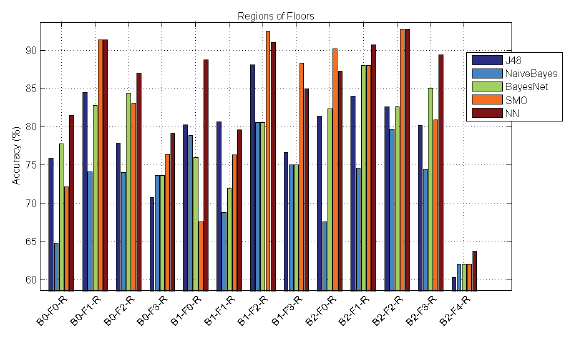
\includegraphics[scale=1]{figures/regionClassification.png}
		\caption{Accuracy results of region classification}
		\label{fig:regionClass} %% NOTE: always label *after* caption!
	\end{center}
\end{figure}

Si les deux tableaux ci-dessous sont analysés, l'algorithme NN est le meilleurs pour tous les dataset niveau temps d'execution. En ce qui concerne la précision, Bayes Net est meilleur pour la classification "building" par contre NN est meilleur dans tous les autres cas.

\begin{figure}[H]
	\begin{center}
		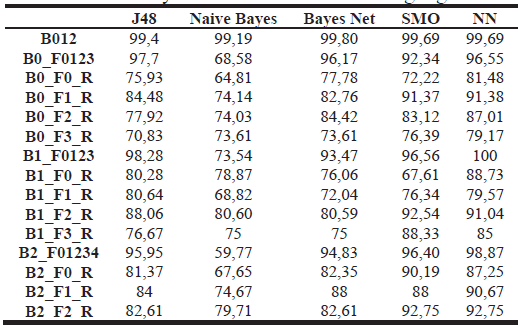
\includegraphics[scale=1]{figures/accuracy.png}
		\caption{Accuracy results of machine learning algorithms}
		\label{fig:accuracy} %% NOTE: always label *after* caption!
	\end{center}
\end{figure}

\begin{figure}[H]
	\begin{center}
		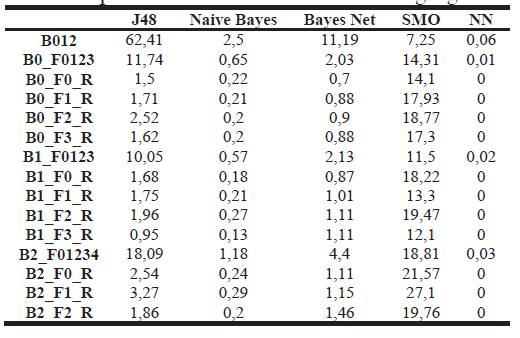
\includegraphics[scale=1]{figures/time.png}
		\caption{Elapsed time results of machine learning algorithms}
		\label{fig:time} %% NOTE: always label *after* caption!
	\end{center}
\end{figure}

De cette publication en découle que NN est supérieur à toutes les autres méthodes pour estimer la position. En outre, J48 offre des performances quasiment identiques lorsqu'il est utilisé avec des algorithmes itératifs, à savoir AdaBoost et Bagging.

\section{Résumé du document 02}
Cette publication traite de la diminution de erreur du mode ranging concernant la localisation UWB (ultra wide band). Plusieurs techniques existent pour diminuer l'erreur de positionnement en détectant ce qui est en ligne de vue (LOS) ou non (NLOS). Ici, il est exploité une autre technique qui va directement diminuer cet erreur que ça soit en LOS ou NLOS. Ils appliquent deux classes de régresseurs non paramétriques pour avoir une estimation de l'erreur de mesure. Afin de valider leurs résultats ils ont fait un vaste campagne de mesures intérieures. Cette technique montre une amélioration de performances significatives dans divers scénarios par rapport aux approches conventionnelles. 

Ils se sont appuyé sur des outils de Machine Learning, et proposent deux techniques de régression non paramétriques pour estimer l’erreur de mesure, en se basant uniquement sur la forme d’onde reçue et la distance estimée.


\begin{enumerate}
	\item La première technique utilise une régression de machine à vecteurs de support (SVM - support vector machine) pour trouver un hyperplan qui se rapproche de l'erreur de mesure en fonction des données d'apprentissage. 
	\item La seconde technique utilise un processus gaussien (GP) pour déterminer la distribution a posteriori de l'erreur de mesure, en fonction des données d'apprentissage. 
\end{enumerate}

L'erreur de mesure estimée, associée à une mesure de certitude, peut être transmise à un algorithme de localisation. Leurs techniques de régression présentent l'avantage supplémentaire de pouvoir être appliquées même lorsque les données d'apprentissage ne sont pas étiquetées avec des informations LOS ou NLOS.

\subsection{Ranging Errors}
Lors de mesure il existe beaucoup de paramètres qui peuvent créer une erreur. Avec un seul model il est difficile de capturer tout les types de perturbations. Dans cette publication, ils se basent sur 1024 mesures (512 LOS et 512 NLOS).

\begin{figure}[H]
	\begin{center}
		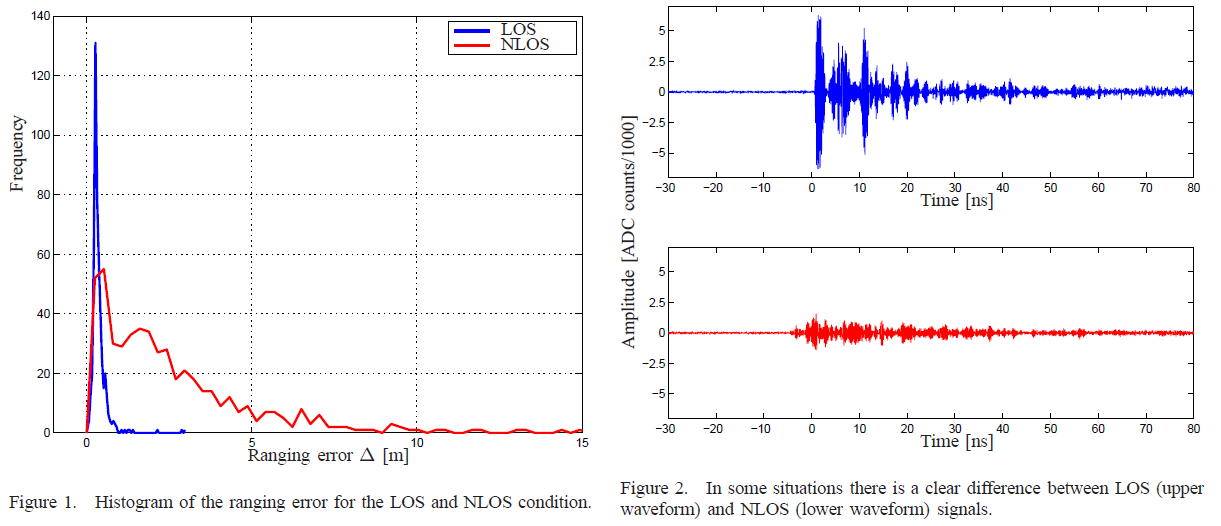
\includegraphics[scale=1]{figures/LosNlos.png}
		\caption{Ranging error - LOS and NLOS}
		\label{fig:LosNlos} %% NOTE: always label *after* caption!
	\end{center}
\end{figure}

Suite, aux différentes mesures et différentes observations dans leur article, ils décident de ne pas labéliser les signaux en LOS et NLOS.

\subsection{Algrorithme}
\subsubsection{Regression with Support Vector Machines}
\subsubsection{Regression with Gaussian Processes}

\subsection{Conclusion}
Les approches classiques pour faire face au défi de la localisation dans des environnements encombrés impliquent généralement d'abord la détection de la condition NLOS, puis la prise de mesures appropriées pour prendre en compte la condition NLOS. Toutefois, la grande variété de matériaux et d’environnements d’exploitation variés peuvent impacter les performances de la mesure de ranging, ce qui indique que la distinction entre LOS et NLOS n’est pas toujours significative. Sur la base de cette observation, ils ont adopté pour une approche différente dans cet article. Leur approche utilise des techniques de Machine Learning non paramétriques (SVM et GP) pour estimer l’erreur de "ranging" directement à partir de la forme d’onde reçue, sans aucune connaissance a priori ou a posteriori de la condition NLOS. 

Sur la base d'une vaste campagne de mesures en intérieur avec des radios UWB conformes à la FCC, ils ont évalué les performances de localisation en termes de probabilité de panne pour différentes stratégies de localisation. Leurs résultats ont révélé que: 

\begin{enumerate}
	\item La minimisation de l1-norme est plus robuste pour faire face aux valeurs aberrantes (outliers) que la minimisation de l2-norme, pour une localisation sans atténuation.
	\item les contraintes peuvent générer des gains significatifs, en particulier lorsque les exigences de localisation ne sont pas trop strictes.
	\item les techniques de régression SVM ou GP offrent des gains de performance supplémentaires pour tous les scénarios considérés.
	\item Les techniques de régression SVM ou GP, combinées à la connaissance des contraintes relatives à l'erreur de "ranging", offrent les meilleures performances pour les scénarios considérés.
\end{enumerate}

\section{Résumé du document 03}
\subsection{Pro/con}
%\chapter{Rapport intermédiaire: 27 août - 18 septembre}
Ce chapitre présente les différentes étapes effectuées lors du déroulement de ce travail entre le 27 août et le 18 septembre 2018 (durée: 3 semaines).

\section{Cahier des charges}
\todo{valider.}

\subsection{Objectifs et tâches à réaliser}
\begin{enumerate}
	\item Etude théorique des réseaux de neuronnes convolutifs
	\item Etude de l'état de l'art de la reconnaissance de piétons
	\item Etude de l'état de l'art de l'utilisation d'images thermiques pour l'entrainement et l'inférence d'un réseau de neuronnes convolutif
	\item Mise en place et tests des exemples du framework Bonseyes\footnote{https://www.bonseyes.com/}
	\item Modification du framework Bonseyes pour permettre l'entrainement d'un réseau de neuronnes avec les images thermiques d'un dataset existant
	\item Evaluation des possibilité et modification du framework Bonseyes pour permettre l'entrainement d'un réseau de neuronnes avec les images thermiques et visibles d'un dataset existant
	\item Eventuellement: mise en place de l'inférence du modèle entrainé pour une reconnaissance en temps réel


\end{enumerate}

\subsection{Délivrables}
\begin{itemize}
	\item Les différentes études précitées
	\item Marches à suivre et résultats de la mise en place des exemples Bonseyes (?)
	\item Version modifiée du framework Bonseyes avec support de l'entrainement utilisant un dataset d'images thermiques et éventuellement visibles
	\item Eventuellement: plateforme de reconnaissance en temps réel
\end{itemize}

\subsection{Délais}
\begin{itemize}
	\item La remise du rapport doit être faite au plus tard le vendredi 8 février 2019.
	\item La défense se déroulera entre le 4 et le 15 mars 2019.
	\item Les tâches obligatoires doivent être finies avant le 1\ier{} juin.
	\item les tâches optionnelles devraient être commencées au plus tard le 15 janvier 2019, afin d'avoir au moins 15 jours pour proposer et tester un concept suffisant.
\end{itemize}


\section{Etat de l'art}
\todo{faire un état de l'art sur la reconnaissance multispectrale de piétons}


\section{Datasets disponibles}
Afin de procéder à l'entrainement du modèle, il est nécessaire de posséder un dataset avec des images aussi proches que possible de celles qui seront fournies lors de l'inférence.

Bien que ce projet porte sur une reconnaissance "multispectrale", il peut être intéressant de tester l'entrainement avec des datasets d'images d'un seul type: thermique ou visible.
En effet, cela peut servir à prendre en main le framework Bonseyes plus facilement, sans avoir à se préoccuper de la fusion des images dès le début.
Cela peut aussi permettre d'entrainer un modèle spécifiquement pour les images soit visibles, soit thermiques en fuisionnant les résultats à la fin.

Pour cela, 4 types de datasets seront pris en considération:
\begin{itemize}
	\item images visibles uniquement,
	\item images thermiques uniquement,
	\item images thermiques et images visibles avec le même cadrage et sans parallaxe,
	\item images thermiques et images visibles avec cadrage différent.
\end{itemize}

Comme ce projet porte sur la reconnaissance des piétons, les datasets utilisés pour l'entrainement devraient posséder les plus de piétons possibles. Dans la pratique, l'entrainement sera fait pour les classes labellisées pour chaque dataset. Il n'y aura donc pas forcément que la reconnaissance des piétons qui sera entrainée, mais potentiellement aussi d'autres classes, telles que les voitures et les vélos.

\subsection{FLIR}
FLIR Systems, un grand fabricant de capteurs et caméras infrarouge a mis a disposition, dès juillet 2018, un dataset contenant des images thermiques ainsi que visbles\footnote{https://www.flir.com/oem/adas/adas-dataset-form/}.
\todo{plus de détails sur l'acquisition, dimensions,...}
Les spécifications de ce dataset sont présentées à la table \ref{tab:dataset-flir}
\begin{table}[h!]
	\begin{center}
		\caption{Caractéristiques du dataset fourni par FLIR}
		\label{tab:dataset-flir}
		\begin{tabular}{p{4.5cm}|p{8cm}}
%			\textbf{Value 1} & \textbf{Value 2}\\ % <-- added & and content for each column
%			\hline
			Description & Images visibles (RGB) et thermiques synchronisées.\\
			& 2 caméras distantes d'environ 5cm pour minimiser la parallaxe\\
			Nombre d'images & > 14'000 provenant de segments de vidéos\\
			Labels & Piétons, voitures, vélos, chiens, autres véhicules\\
			Nombre d'annotations: & 10'228 dont 9214 avec encadrement (bounding box)\\
			Nombre de: piétons & 21'965 \\
			Nombre de voitures & 12'013\\
			Nombre de vélos & 1205\\
			Nombre de chiens & 0\\
			Nombre d'autres véhicules & 540 \\
%			1 & 1110.1 \\ % <--
%			2 & 10.1\\ % <--
%			3 & 23.113231\\ % <--
		\end{tabular}
	\end{center}
\end{table}

Ce dataset peut être téléchargé gratuitement après s'être enregistré sur le site de FLIR.

\subsection{Kaist}

KAIST\footnote{Korea Advanced Institute of Science and Technology} a développé un dataset particulièrement intéressant, comportant des images visibles ainsi que des images thermiques.

Ce dataset est disponible en ligne\footnote{http://rcv.kaist.ac.kr/multispectral-pedestrian/}, gratuitement, après enregistrement.
\todo{lire et résumer CVPR15}
Les spécifications de ce dataset sont:
\begin{itemize}
	\item 95 328 paires d'images thermiques et visibles, alignées, sans parallaxe,
	\item 103 128 annotations de piétons, avec bounding box,
	\item 1182 piétons différents.
\end{itemize}

\begin{table}[h!]
	\begin{center}
		\caption{Caractéristiques du dataset fourni par KAIST - comparaison des deux caméras}
		\label{tab:dataset-kaist2}
		\begin{tabular}{p{4.5cm}|p{5cm}|p{5cm}}
			\textbf{Description} & \textbf{Caméra visible (RGB)} & \textbf{Caméra thermique}\\
			\hline
			Modèle de caméra & PointGrey Flea3 & FLIR A35\\
			Dimension des images & 640x480 & 320x256\\
			Champ de vue & 103.6\degres vertical & 39\degres vertical\\
		\end{tabular}
	\end{center}
\end{table}

\section{Modèles disponibles?}


\section{Deep learning}


\section{CNN}


\section{Bonseyes}
Bonseyes est une plateforme d'intelligence artificelle, développé dnas le cadre d'un projet Horizon 2020.\todo{détailler!}
Le but de Bonseyes est de mettre à disposition des utilisateurs une plateforme modulable pour l'utilisation du deep-leanring.
Cette plateforme, en développement actuellement devrait permettre:
\begin{itemize}
	\item Utilisation de différents frameworks tels que Tensorflow, Caffe, Theano\dots
	\item Utilisation de plugins pour effectuer les calculs sur DSP, FPGA, GPU ou CPU.
\end{itemize}


\subsection{Prérequis et dépendances}
Bonseyes, grâce à un concept de workflows utilisant des conteneurs Docker permet une installation simple.

Les différents éléments requis sont:
\begin{itemize}
	\item Un PC possédant une carte graphique Nvidia,
	\item Une distribution GNU/Linux,
	\item Docker
	\item Nvidia-docker
	\item Drivers Nvidia
	\item git
\end{itemize}	

\subsection{Architecture}

\todo{parler de l'architecture, des tools, workflows,...}

\subsection{Installation des dépendances et de be-admin}
Afin de pouvoir utiliser les différents workflows existant et en développer de nouveau, il est nécessaire d'installer les dépendances de base de Bonseyes ainsi que d'installer l'outil 'administration des workflows (be-admin).

Dans cet exemple, ces instructions s'appliquent à une machine fonctionnement sur Ubuntu 16.04 LTS.

Installation des drivers nvidia
\begin{lstlisting}
sudo add-apt-repository ppa:graphics-drivers/ppa
sudo apt-get update
sudo apt-get install nvidia-384
\end{lstlisting}

Installation de git, docker et nvidia-docker
\begin{lstlisting}
sudo apt-get update
sudo apt-get install git docker nvidia-docker
\end{lstlisting}




\subsection{Execution du workflow MNIST}

Le jeu de données MNIST\footnote{Modified National Institute of Standards and Technology} est une compilation de 70 000 images de chiffres manuscrits. Ce dataset convient particulièrement bien pour différents tests, tels que la vérification du bon fonctionnement de Bonseyes, car c'est un dataset assez simple, contenant des images de faibles dimensions\footnote{28x28 pixels} avec un nombre restreint de classes\footnote{10 classes représentant les chiffres de 0 à 9}.

Afin de pouvoir procéder à ces tests, il existe dans le projet Bonseyes, un sous-projet appelé "wp3-project-mnist" qui est l'implémentation de l'entrainement et du test d'un MLP\footnote{Multilayer Perceptron} utilisant le dataset MNIST.



Les instructions pour la mise en place et l'exécution de ce workflow se trouvent à l'adresse \url{https://bitbucket.org/bonseyes/wp3-project-mnist/src/master/}

\begin{lstlisting}
{
	"application_config" : {
		"run_opts": {
			"volumes": {
				"nvidia_driver_384.130": { "bind": "/usr/local/nvidia", "mode": "ro"}
			},
			"devices": [
			"/dev/nvidiactl",  "/dev/nvidia-uvm-tools", "/dev/nvidia-uvm", "/dev/nvidia0"
			]
		}
	}
}
\end{lstlisting}

\subsection{Execution du workflow Object Detection}

\section{Utilisation du dataset Kaist dans le framewrok object detection}

%\chapter{Introduction et contexte}
\Blindtext
%\chapter{Définition d'une base réflexion pour un protocole sécurisé sur un bus CAN}
\blindtext

\lstset{
	language=C,
	showstringspaces=false,
	basicstyle=\ttfamily\small,
	commentstyle=\itshape,
	morecomment=[s]{"""}{"""},
}
\lstinputlisting[caption={Exemple d'écriture en boucle d'une trame CAN en utilisant le framework Python "pyvit" - code source}, label={lst:sample}]{source_code/sample.c}

\section{Buts}
\blindtext

\begin{itemize}
	\item La taille des données pouvant être transmises doit être plus grande que 8 bytes \footnote{Taille maximum du champ de données sur le bus CAN 2.0A/B} afin de pouvoir contenir une signature, car habituellement une signature a une taille d'au moins une centaine de bits au minimum.
	\item Chaque émetteur de données doit pouvoir signer ses messages avec une clé privée.
	\item Chaque récepteur de données doit pouvoir vérifier les messages reçus avec une clé publique qui doit être autorisée par un élément central auquel il a été décidé de faire confiance.
	\item Les clés publiques doivent être stockées chez un gestionnaire de clés publiques, afin de pouvoir modifier les périphériques autorisés à envoyer des messages aisément.
\end{itemize}

\subsection{Paquet CAN standard}
Lors de l'utilisation de la surcouche CanSecure, chaque paquet de 8 bytes envoyé sur le bus CAN comporte les données suivantes dans son champ de données (voir figure \ref{fig:pack-can}):
\begin{itemize}
	\item byte 0: frame ID
	\item byte 1: packet number
	\item bytes 2-7: data (6 bytes)
\end{itemize}

Le champ "frame ID" permet d'identifier un paquet CanSecure.\\
Le champ "packet number" permet d'identifier l'emplacement du paquet fragmenté dans le paquet CanSecure.\\
Le champ "data" permet d'envoyer 6 bytes de données utiles du paquet CanSecure.

\myfig{CanSecure/pack-can-2.png}{0.8}{Paquet CAN standard}{fig:pack-can}
\FloatBarrier

\paragraph{Dans le meilleur des cas:}
Lors de l'envoi de 1404 bytes de données, avec le périphérique recevant les données ayant déjà la clé publique en cache, il faut transmettre $\lceil\frac{1404+132}{6}\rceil=256$ paquets CAN.\\
Chaque paquet CAN a une taille de 108 bits (CAN 2.0A, 64 bits de données, en omettant le bit stuffing).\\
Cela implique donc de transférer $256*108 = 27648$bits $= 3456$bytes.\\
Ce qui donne donc: $overhead = \frac{3456}{1404} = 2.46$.


C'est la raison pour laquelle, dans le protocole TLS, les deux parties (client et serveur) commencent tout d'abord par une phase de "handshake" permettant au client et au serveur de s'échanger des clés publiques et des certificats, puis un secret partagé est généré, permettant un fonctionnement à base de cryptographie à clés privées, voir \cite{rfc5246}, même si chaque paquet comporte néanmoins très souvent une signature à base de clé publique.

%\chapter{Conclusion}

Durant ce projet, une analyse poussée du fonctionnement d'un bus CAN a pu être faite, permettant de mettre en évidence le fait que ce bus avait été prévu à l'origine pour permettre une grande résistance vis-à-vis des perturbations électriques et permettant une hiérarchie stricte des émetteurs de messages visant un système à faible latence et haute fiabilité. Cependant, le développement de ce bus n'avait pas pris en compte la présence possible d'un acteur malveillant et aucune sécurité visant à préserver l'intégrité ni l'authenticité des messages n'a été prévue dans la norme.

Ce travail a permis d'analyser l'architecture du véhicule, afin de comprendre quels types de messages et quelles informations circulent sur quels bus et l'ont peut voir que l'entreprise Navya a pris en compte certains points importants, tels que l'utilisation de plusieurs bus permettant de séparer les informations à transmettre.

Cependant, cela n'est pas suffisant; il n'y a pas de redondance de l'information. Si l'un des bus ne permet plus une communication, les informations qui devaient transiter sur ce bus n'ont pas de cheminement alternatif et le flux d'informations est rompu. Dans le cadre d'un véhicule autonome circulant à basse vitesse, cela peut être perçu comme un incident peu grave, et le véhicule détectant une anomalie peut effectuer un freinage d'urgence. Il serait néanmoins intéressant de permettre une redondance de l'information permettant d'éviter cela.

Lors de l'analyse du véhicule autonome, il a aussi pu être confirmé le fait que les messages concernant par exemple les commandes de direction transitent en clair et sans signature.
Cela implique donc que le récepteur du message n'a aucun moyen de vérifier leur provenance.

Concernant la protection de l'authenticité et de la provenance des données, il ne semble pas y avoir à l'heure actuelle, beaucoup de surcouches pour le bus CAN permettant d'assurer cette authenticité afin d'empêcher un attaquant de fournir de fausses données. Cela est le problème le plus grave, et c'est pourquoi une base de protocole "CanSecure" est décrite dans ce document. Ce "CanSecure" n'est pas prévu pour être implémenté tel quel, mais vise à suggérer une piste de réflexion sur la problématique de l'authenticité des données et sur un moyen possible d'y remédier.

% following structure:
%	000 => 099 abstract, acknoledgements,...
%	100 => 899 content
%	900 => 999 annexes, ...


%----------------------------------------------------------------------------------------
%	Bibliography
%----------------------------------------------------------------------------------------

%% prints every entry of the bib file -- useful in a state where is no cite
\appendix
\nocite{*}
\printbibliography

%----------------------------------------------------------------------------------------
%	Appendix
%----------------------------------------------------------------------------------------
%% add possible appendix
%\appendix
%\addpart*{Appendix}
%\chapter{Planning}
\begin{figure}[htp]
	\begin{center}
		\includegraphics[width=1\textwidth, angle=90]{../figures/pictures/000-planning.png}
		\caption[Planning]{Planning}
		\label{fig:planning} %% NOTE: always label *after* caption!
	\end{center}
\end{figure}





%----------------------------------------------------------------------------------------
%	\end{document}
%----------------------------------------------------------------------------------------
\end{document}
